\begin{frame}{Sostenibilità e AI} 
        \begin{itemize}
                \item \emoji{recycle} \textbf{Sostenibilità}: Capacità di soddisfare i bisogni delle generazioni presenti senza compromettere le generazioni future. Esempio di impegno è l'Agenda 2030 dell'ONU.
                \begin{figure}[H]
                        \centering
                        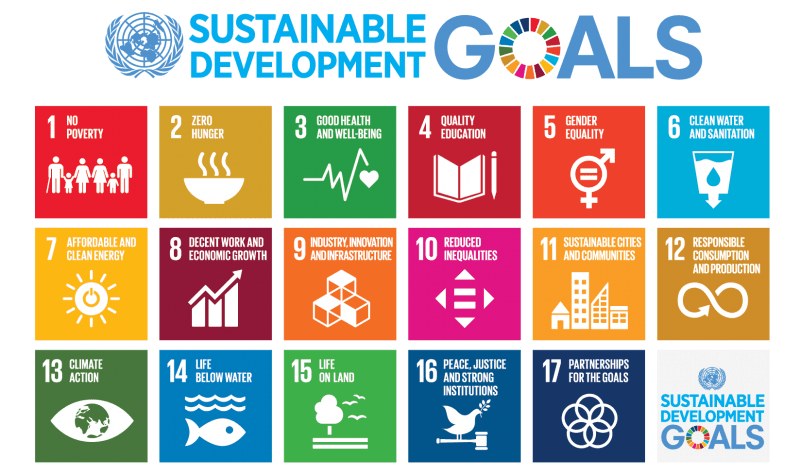
\includegraphics[scale=0.15]{images/sdg.png}
                \end{figure}
                \item \emoji{globe-showing-europe-africa} \textbf{Sostenibilità ambientale}: Uno degli aspetti della sostenibilità. Riduzione delle emissioni di CO2, rispetto delle risorse naturali e dell'ambiente.
                \item \emoji{seedling} \textcolor{green}{Green AI}: Durante l'addestramento si considera l'impatto ambientale in termini di emissioni di CO2 e consumo di energia.
                \item \emoji{factory} \textcolor{red}{Red AI}: non considerara l'impatto ambientale (massime prestazioni)
        \end{itemize}
\end{frame}
